\documentclass{article}
\usepackage[paperwidth=6in, paperheight=9in, margin=0.75in]{geometry}
\usepackage{fontspec}
\usepackage{xcolor}
\usepackage{graphicx}
\usepackage{tikz}

% Set up fonts
\setmainfont[Script=Devanagari] {Tiro Devanagari Marathi}
\newfontfamily\devanagarifont[Scale=MatchUppercase]{Tiro Devanagari Marathi}

\newfontfamily\devtransl[Mapping=DevRom]{Segoe UI}
\graphicspath{{images/}}

% Define colors
\definecolor{titleorange}{RGB}{255,140,0}
\definecolor{subtitleblue}{RGB}{0,51,102}
\definecolor{authorgreen}{RGB}{0,102,51}

\pagestyle{empty}

\begin{document}

% FRONT COVER PAGE
\thispagestyle{empty}
\null\vfill

\begin{center}
% Title - big orange font, 60% page width
{\fontsize{64}{78}\selectfont\color{titleorange}\textbf{सहज जीवन}}

\vspace{1em}

% Subtitle - quarter size, dark blue
{\fontsize{10}{14}\selectfont\color{subtitleblue}(मराठीतील पहिले मुक्त-स्रोत, सार्वजनिक, सहकारी आणि अद्ययावत पुस्तक)}

\vspace{10em}

% Author - dark green
{\fontsize{12}{14}\selectfont\color{authorgreen}\textbf{अनुवादक-लेखक}}

\vspace{1em}

{\fontsize{18}{20}\selectfont\color{authorgreen}\textbf{\ldots आणि  डॉ. योगेश हरिभाऊ कुलकर्णी}}
\end{center}

\vfill\null
\clearpage

% BACK COVER PAGE
\thispagestyle{empty}
\vspace*{0.5in}

% Book description
\noindent\textbf{पुस्तकाविषयी:} हे पुस्तक प्रामुख्याने दोन भागात आहे.  पहिल्या भागात लीओ बाबाउटा यांच्या 'द एफर्टलेस लाईफ' या पुस्तकाचा स्वैर अनुवाद आहे.  हे मूळ पुस्तक जगभरातील लेखकांच्या-वाचकांच्या मदतीने सार्वजनिक पद्धतीने लिहिले गेले होते.  मूळ इंग्रजीतील पुस्तकप्रमाणेच  हे मराठी भाषांतरसुद्धा  कोणत्याही प्रकाशन हक्काधिकाराशिवाय (Uncopyrighted) उपलब्ध ठेवले आहे.  दुसऱ्या भागात पुस्तक स्वरूपात डॉ. योगेश हरिभाऊ कुलकर्णी यांचे विचार आहेत.  हा दुसरा भाग ऑनलाईन वर अद्ययावत (live) असणार आहे.  म्हणजेच GitHub repository मध्ये इतर लेखक-वाचकांचे विचार सुद्धा सम्मिलीत केले जात आहेत. याचा सर्व प्रपंचाचा उद्देश मराठी वाचकांना ``सहज जीवन'' जगण्यासाठी मार्गदर्शन मिळावे हा आहे. 

\vspace{1.5em}

% Target audience
\noindent\textbf{वाचकांविषयी:} स्वसंवर्धनात रस असणाऱ्या सर्वांसाठी हे पुस्तक योग्य आहे.

\vspace{1.5em}

% Author bio
\noindent\textbf{अनुवादक-लेखक-प्रकाशक-संकलकाविषयी: डॉ. योगेश हरिभाऊ कुलकर्णी} हे तंत्रज्ञान क्षेत्रातील अनुभवी अभ्यासक आहेत. त्यांना कृत्रिम बुद्धिमत्ता, मशीन लर्निंग आणि डेटा सायन्स या क्षेत्रात अनेक वर्षांचा अनुभव आहे. शैक्षणिक क्षेत्रात तसेच उद्योगात काम करून त्यांनी या विषयावर व्यापक अभ्यास केला आहे. त्यांचे पूर्वीचे लेखन कार्य आणि संशोधन हे मराठी भाषेत तंत्रज्ञान विषयक साहित्याला वाव देण्याच्या दिशेने योगदान आहे.

\vfill

% Author photo and contact info at bottom
\begin{tabular}{@{}p{0.3\textwidth}@{}p{0.2\textwidth}@{}p{0.3\textwidth}@{}}
\centering
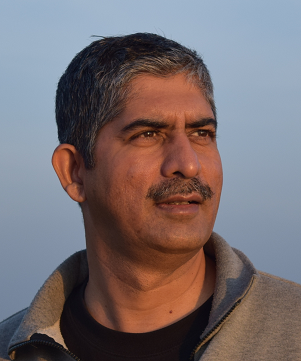
\includegraphics[width=\linewidth,keepaspectratio]{myphoto} 

yogeshkulkarni@yahoo.com
&
% blank column &
& 
\centering
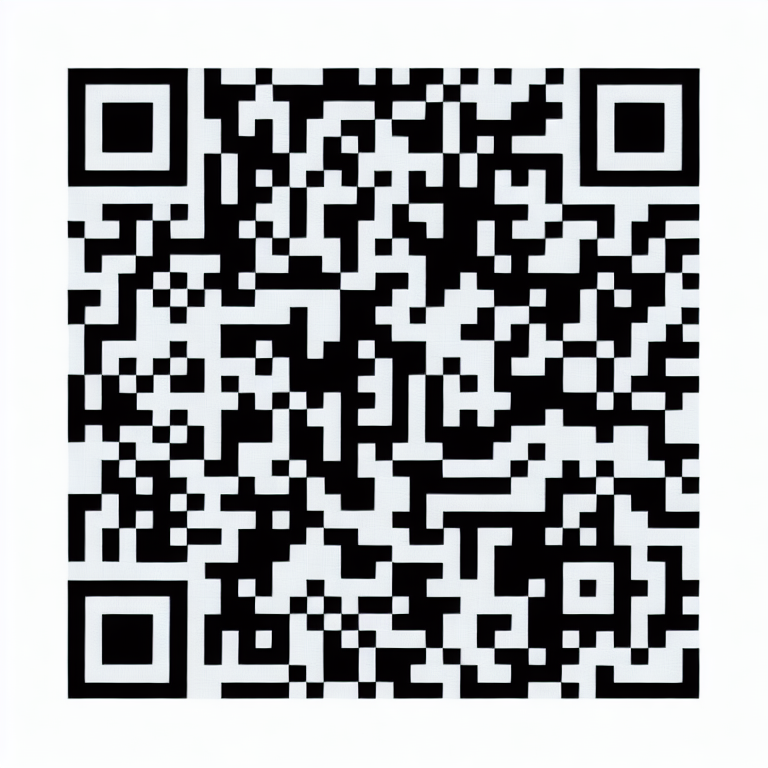
\includegraphics[width=\linewidth,keepaspectratio]{mylinkedinqr}

+91 9890251406
\end{tabular}


% % Publisher info at bottom
% \begin{center}
% \textbf{प्रकाशन मंच (Publishing Platform) }\\
% \texttt{www.notionpress.com}\\
% %ISBN: [ISBN नंबर]
% \end{center}

% \begin{center}
% 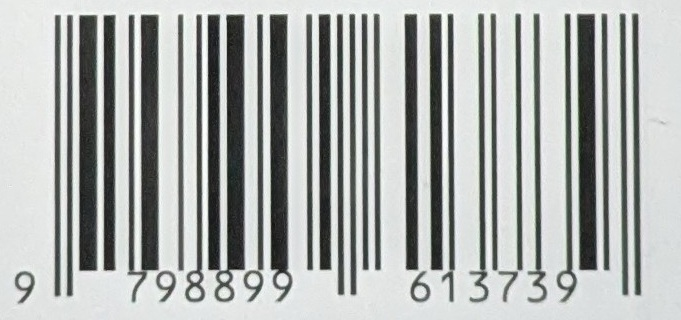
\includegraphics[width=3cm]{sahajjeevan_isbn}
% \end{center}

\end{document}